\section{User management}
\label{sec:USR_user_management}

The application list addressed to a community of users / customers have to implement the management mechanisms of the user.

The mechanisms for base user management are:
\begin{itemize}
\item user login 
\item user signup
\item user logout
\item user management
\end{itemize}
To these advanced management mechanism may be associated, such as:
\begin{itemize}
\item email verification 
\item email changing  
\item password recovery/reset 
\item password changing  
\end{itemize}

The mechanisms of advanced management, involving the use of email, must necessarily be based on a email management service.
Challenge of this project is to be able to encapsulate these mechanisms / behaviors in their elements, to allow it to integrate user management with the same ease with which it is possible to insert HTML elements on a page.

\subsection{User Management services}
\label{subsec:USR_user_management_services}
This section talks about the various existing services for user management as: Stormpath, Userapp and Auth0.
\subsubsection{Stormpath}

Stormpath is a User Management API that reduces development time with instant-on, scalable user infrastructure. Stormpath's intuitive API and expert support make it easy for developers to authenticate, manage and secure users and roles in any application.

Stormpath,it has a simple goal: give developers a complete user management system, so can focus on building great applications.\cite{usr_stormpath}

\begin{itemize}
\item Pre-built authentication \& authorization.
\item Schemaless, secure user data \& profiles.
\item Code-free Active Directory, Facebook \& Google login.
\item Open Source SDKs \& complete sample apps.
\end{itemize}

\begin {figure}[h]
\graphicspath{{images/chapter_USR/}}
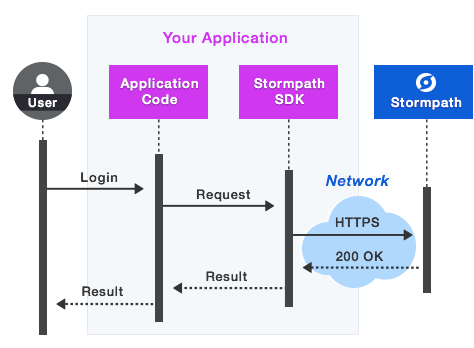
\includegraphics[width=\textwidth]{stormpath}
\caption{Stormpath User Management API}
\end {figure}

\subsubsection{Userapp}

UserApp is a cloud-based user management API for web apps. The purpose is to relieve developers from having to program logic for login, sign up, calculate payments, turn on or off features, etc. And instead focus on their core product.

UserApp provides with user management functionality that results in faster development, faster revenue, more users, and the ability to serve users better by engaging with them more efficiently.\cite{usr_userapp}

\begin{itemize}
\item User authentication - Have the user authentication ready today. It is possible just a few lines of code away with one of SDKs.
\item One-click integrations - Integrate the users with third-party services with just one click.
\item Mobile, web, and server - No matter where is need to integrate the user authentication, it got  covered.
\end{itemize}

\subsubsection{Auth0}

Auth0 is an enterprise-grade platform for modern identity.
Auth0 give the tools that eliminate the friction of authentication for the applications and APIs - all accessible through the account dashboard.\cite{usr_auth0}

\begin {figure}[h]
\graphicspath{{images/chapter_USR/}}
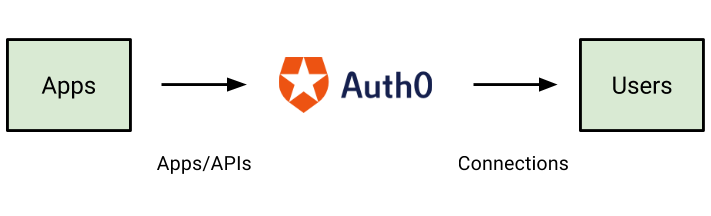
\includegraphics[width=\textwidth]{auth0}
\caption{Auth0 Overview}
\end {figure}

It is possible connect any application, written on any language or stack to Auth0, and separately define how users of that application authenticate:

\begin{itemize}
\item Custom credentials: username/passwords.
\item Social network logins: Google, Facebook, Twitter and any OAuth2 or OAuth1 provider.
\item Enterprise directories: LDAP, Google Apps, Office 365, ADFS, AD, SAML-P, WS-Federation, etc.,
\item Password-less systems: TouchID, one time codes on SMS.
\end{itemize}


\subsection{User Management Standard API in StrongLoop LoopBack}

X-project is based on StrongLoop LoopBack on the server side.
LoopBack's built-in User model provides essential user management features such as:
\begin{itemize}
\item Registration and confirmation via email.
\item Login and logout.
\item Creating an access token.
\item Password reset. 
\end{itemize}
In general can extend the User model to suit specific needs, so in most cases, it is don't need to create the own User model from scratch.
By default, a LoopBack application has a built-in User model defined by user.json
In particular, it was implemented the connection with MailChimp service, named Mandrill.

\subsection{User Management remote methods}

In addition to the standard APIs, remote methods for email and password changing have been implemented. 

\subsubsection{Change Email}

\begin{lstlisting}[language=html]
Author.change_email = function (new_email, confirm_email, password, cb) {
    if (new_email !== confirm_email) {
      cb({ error: 'email not confirmed' }, null);
      return;
    }

    var userId = getCurrentUserId();  

    Author.findById(userId, function (err, user) {
      if (err) {
        cb(err, null);
        return;
      }

      user.hasPassword(password, function (err, match) {
        if (!match) {
          cb({ error: 'invalid password' }, null);
          return;
        }

        user.updateAttribute('email', new_email, function (err, user) {
          if (err) {
            cb(err, null);
            return;
          }

          cb(null, true);
        });
	  });       
	});
};
   Author.remoteMethod('change_email', {
    http: { path: '/change_email', verb: 'post' },
    accepts: [
      { arg: 'new_email', type: 'string' },
      { arg: 'confirm_email', type: 'string' },
      { arg: 'password', type: 'string' }
    ],
    returns: { arg: 'changed', type: 'boolean' }
  });
\end{lstlisting}

\subsubsection{Change Password}

\begin{lstlisting}[language=html]
Author.change_password = function (new_password, confirm_password, password, cb) {
    if (new_password !== confirm_password) {
      cb({ error: 'password not confirmed' }, null);
      return;
    }

    var userId = getCurrentUserId();  

    Author.findById(userId, function (err, user) {
      if (err) {
        cb(err, null);
        return;
      }

      user.hasPassword(password, function (err, match) {
        if (!match) {
          cb({ error: 'invalid password' }, null);
          return;
        }

        user.updateAttribute('password', new_password, function (err, user) {
          if (err) {
            cb(err, null);
            return;
          }

          cb(null, true);
        });
	  });       
    });
  };
   
  Author.remoteMethod('change_password', {
    http: { path: '/change_password', verb: 'post' },
    accepts: [
      { arg: 'new_password', type: 'string' },
      { arg: 'confirm_password', type: 'string' },
      { arg: 'password', type: 'string' }
    ],
    returns: { arg: 'changed', type: 'boolean' }
  });
\end{lstlisting}


